% !TEX root = 0-main.tex

% \begin{table}
%   \caption{Description of Datasets}
%   \label{table:datasets}
%   \centering
%   \begin{tabular}{llll}
%     \toprule
%     Name     & Size & Distance Metric & Dimensionality \\
%     \midrule
%     MNIST & 70000  & $l_2$, cosine distance  & 784     \\
%     % MNIST & 70000  & cosine distance & 784     \\
%     scRNA-seq & 40000  & $l_1$ & 10170     \\
%     % scRNA-PCA & 40000  & $L2$ & 10     \\
%     HOC4 & 3,360  & Tree edit distance & $\infty$     \\
%     \bottomrule
%   \end{tabular}
% \end{table}


\section{Empirical Results \label{sec:exps}}

We run experiments on three real-world datasets to validate the expected behavior of \algnamenospace: the MNIST hand-written digits dataset \cite{lecun1998gradient}, the 10x Genomics 68k PBMCs scRNA-seq dataset \cite{zheng2017massively} (\url{support.10xgenomics.com/single-cell-gene-expression/datasets}), and the Code.org Hour Of Code \#4 (HOC4) coding exercise submission dataset (\url{code.org/research}), all of which are publicly available.

\paragraph{Datasets.} The MNIST dataset \cite{lecun1998gradient} consists of 70,000 black-and-white images of handwritten digits, where each digit is represented as a 784 dimensional vector. On MNIST, We consider two distance metrics, namely $l_2$ distance and cosine distance.
The scRNA-seq dataset contains the gene expression levels of 10,170 different genes in each of 40,000 cells after standard filtering. On scRNA-seq, we consider $l_1$ distance, which is recommended \cite{ntranos2016fast}.
The HOC4 dataset from Code.org \cite{hoc4dataset} consists of 3,360 unique solutions to a block-based programming exercise on Code.org. Solutions to the programming exercise are represented as abstract syntax trees (ASTs), and we consider the tree edit distance to quantify the similar between solutions. 

\paragraph{Setup.} In Subsec. \ref{subsec:loss}, we show that \algname returns the same results as PAM. We also compare the clustering loss with that of other popular $k$-medoids clustering algorithms \eqref{eqn:total-loss}, including FastPAM \cite{schubert2019faster}, CLARANS \cite{ng2002clarans}, and Voronoi Iteration \cite{park2009simple}. 
In Subsec. \ref{subsec:scaling}, we demonstrate that \algname scales linearly in the number of samples $n$ for all datasets and all metrics considered. 
Each parameter setting was repeated $10$ times with data subsampled from the original dataset.
95\% confidence intervals are provided. 

% In all plots, points are plotted on a log-log scale. individual points represent different random samples of size $n$ drawn from the dataset (if $n = n_{\text{max}}$, the points are only shuffled between runs). Jitter has been added to the x-coordinates for clarity, and a line of best fit has also been overlaid.

% In all plots, points are plotted on a log-log scale. individual points represent different random samples of size $n$ drawn from the dataset (if $n = n_{\text{max}}$, the points are only shuffled between runs). Jitter has been added to the x-coordinates for clarity, and a line of best fit has also been overlaid.

\begin{figure}[ht]
\label{fig:losses}
    \begin{subfigure}{.35\textwidth}
        \centering
        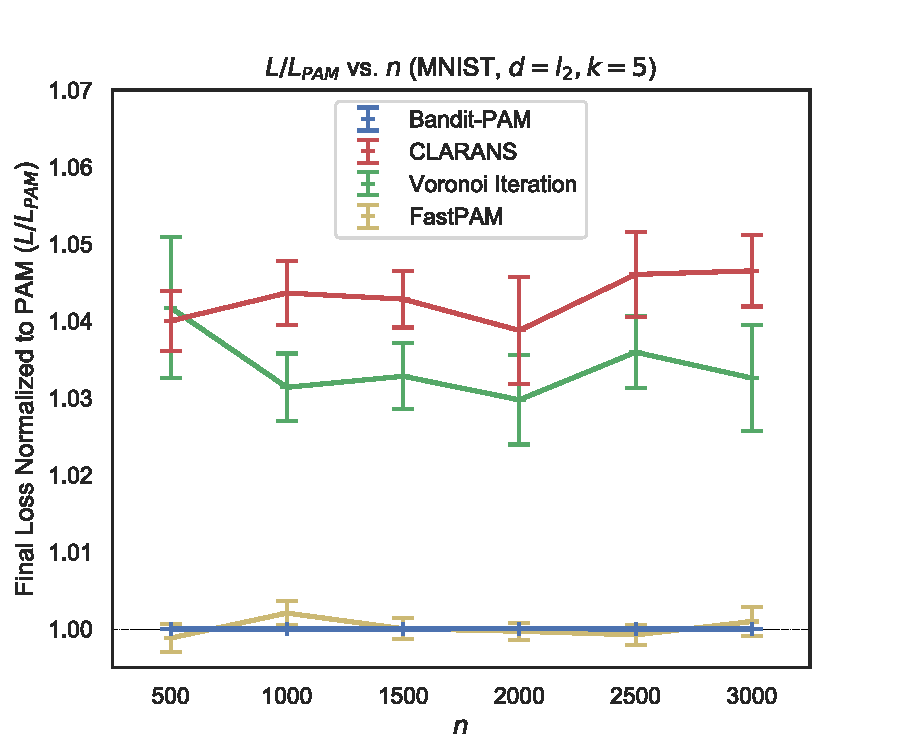
\includegraphics[width=\linewidth]{figures/loss_plot.pdf} 
        \caption{}
    \end{subfigure}
    \begin{subfigure}{.3\textwidth}
      \centering
      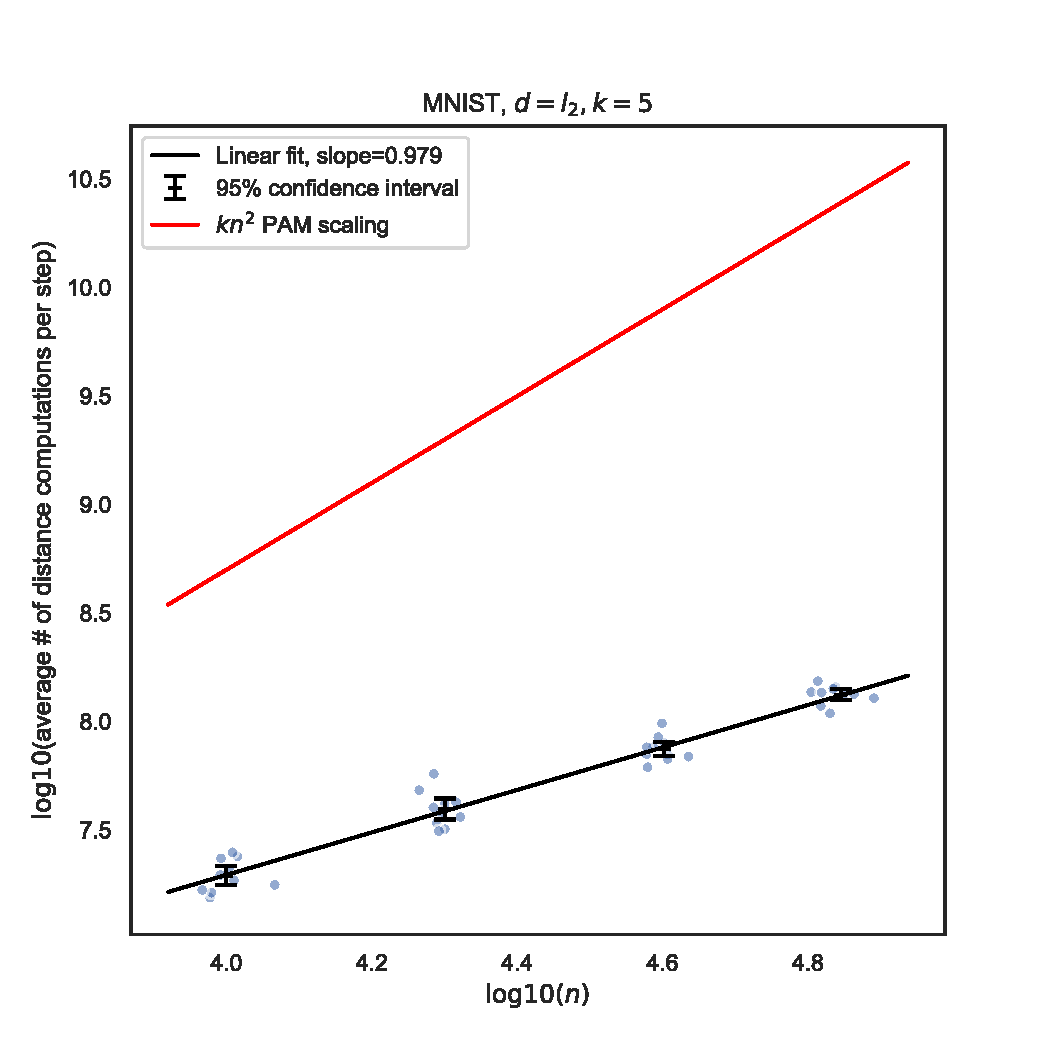
\includegraphics[width=\linewidth]{figures/MNIST-L2-k5.pdf}  
      \caption{}
    %   \label{fig:mods1}
    \end{subfigure}
    \begin{subfigure}{.3\textwidth}
      \centering
      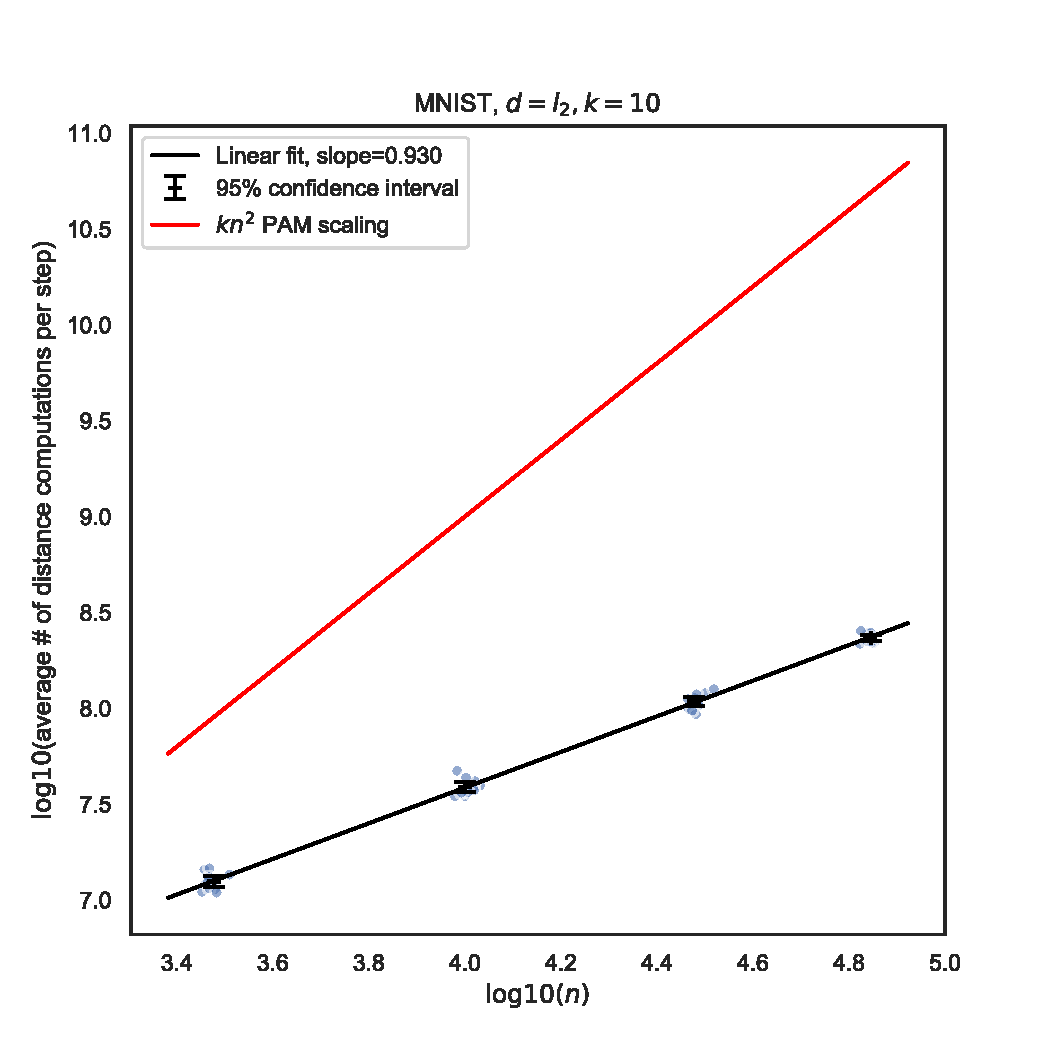
\includegraphics[width=\linewidth]{figures/MNIST-L2-k10.pdf}   
      \caption{}
    %   \label{fig:mods2}
    \end{subfigure}
    \caption{(a) Clustering loss relative to the PAM loss. Data is subsampled from MNIST, sample size $n$ varies from $500$ to $3000$, $k = 5$ and 95\% confidence intervals are provided. \algname always returns the same solution as PAM and hence has loss ratio $1$. FastPAM has a comparable performance, while the other two algorithms are significantly worse. 
    (b-c) Average number of distance calls per iteration vs sample size $n$ for MNIST and $l_2$ distance with (b) $k=5$ and (c) $k=10$. The plot is shown on a log-log scale. Lines of best fit (black) are plotted, as are reference lines demonstrating the expected scaling of PAM (red).}
    \label{fig:mods}
\end{figure}

\subsection{Clustering/loss quality \label{subsec:loss}}

%Baselines: PAM, CLARANS/CLARA, FastPAM, Voronoi Iteration
%The results from section \ref{Nscaling} show that each substep \algname scales almost linearly in dataset size. %Naturally, one might ask if there is a concession in final clustering quality that must be made for the $O(n/\log n)$ speedup of \algname. 

Figure \ref{fig:mods} (a) shows the relative losses of algorithms with respect to the loss of PAM. 
\algname and three other baselines, namely FastPAM \cite{schubert2019faster}, CLARANS \cite{ng2002clarans}, and Voronoi Iteration \cite{park2009simple}. 
We note that FastPAM is different from the FastPAM1 mentioned before; FastPAM takes $O(n^2)$ for each SWAP step but does not guarantee the same solution as PAM. 
\algname always returns the same solution as PAM and hence has loss ratio $1$. FastPAM has a comparable performance, while the other two algorithms are significantly worse. 

% normalized to the loss of PAM for various random subsets of MNIST.
% We observe that \algname finds solutions of equivalent quality to PAM, as does FastPAM, and that these solutions are better than the other baselines. 
% Indeed, in 59 of the 60 experiments, \algname tracks the exact optimization path and returns the exact same results as PAM; the single discrepancy arises in a single SWAP iteration of several hundred, which is in line with our choice of $\delta$.


% \algname always returns the same solution as PAM and hence has loss ratio $1$. FastPAM has a comparable performance, while the other two algorithms are significantly worse. 

% \mo{Need to describe hyperparameters for CLARANS?}


\subsection{Scaling with \texorpdfstring{$n$}{Lg} for different datasets, distance metric, and \texorpdfstring{$k$}{Lg} values \label{subsec:scaling}}

\begin{figure}[ht]
\begin{subfigure}{.33\textwidth}
  \centering
  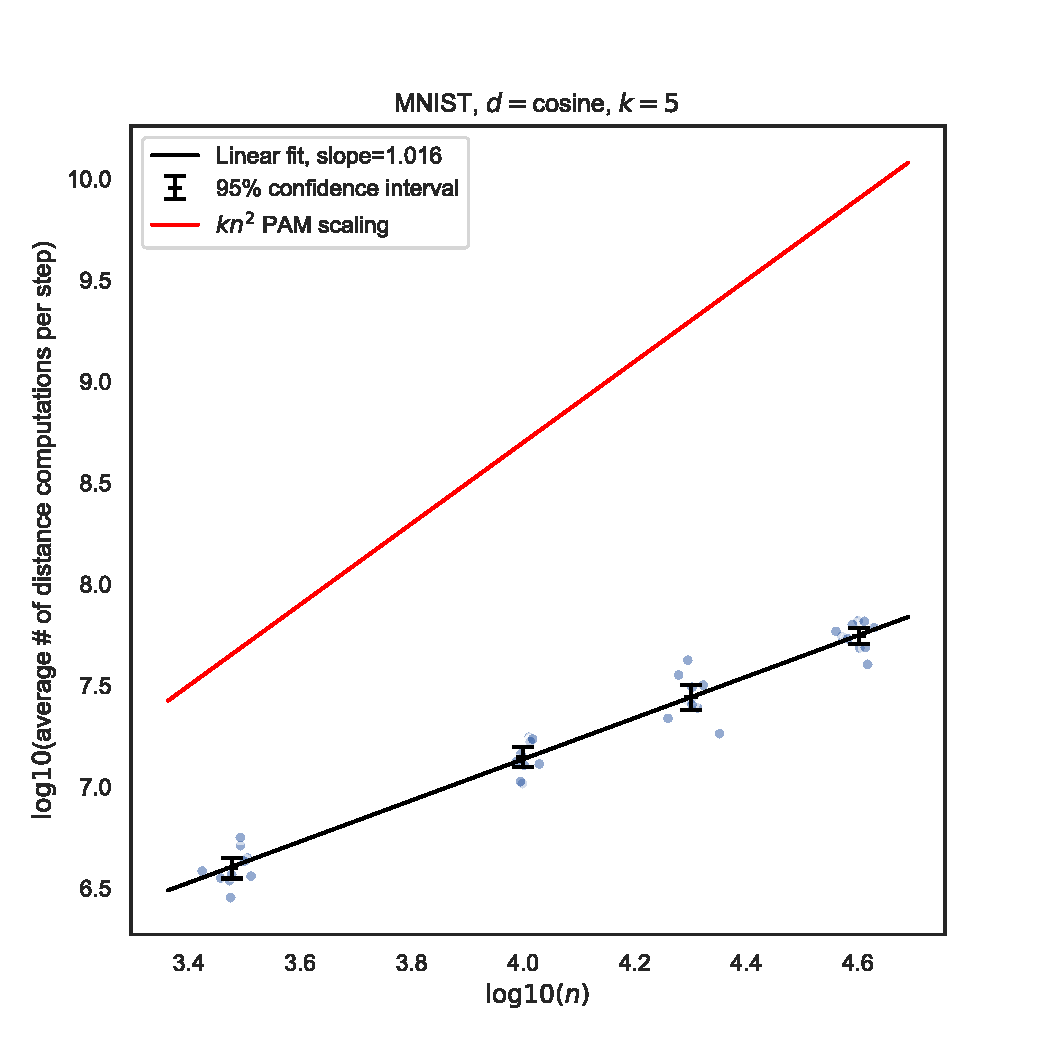
\includegraphics[width=\linewidth]{figures/MNIST-cosine-k5.pdf}  
  \caption{}
  \label{fig:scaling1}
\end{subfigure}
\begin{subfigure}{.33\textwidth}
  \centering
  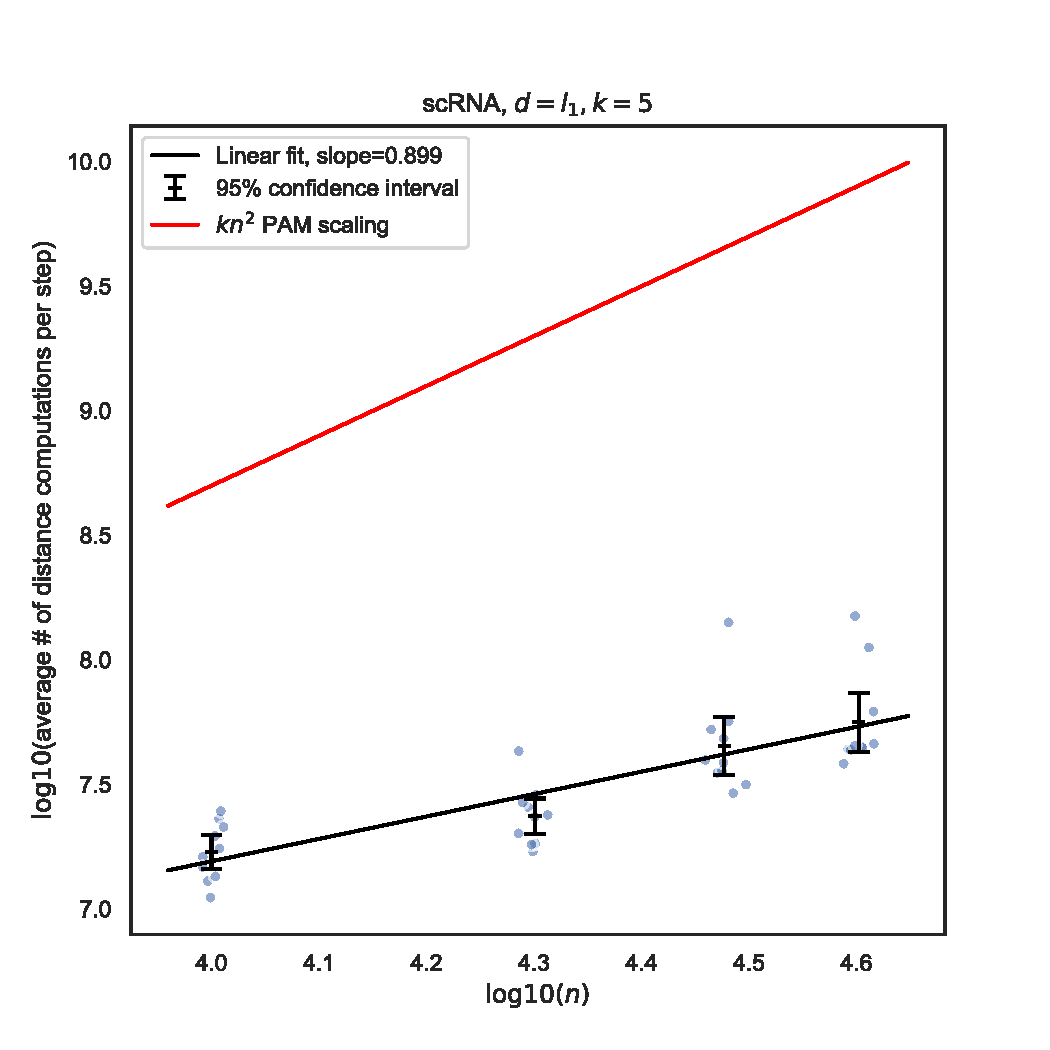
\includegraphics[width=\linewidth]{figures/SCRNA-L1-k5.pdf}   
  \caption{}
  \label{fig:scaling2}
\end{subfigure}
\begin{subfigure}{.33\textwidth}
  \centering
  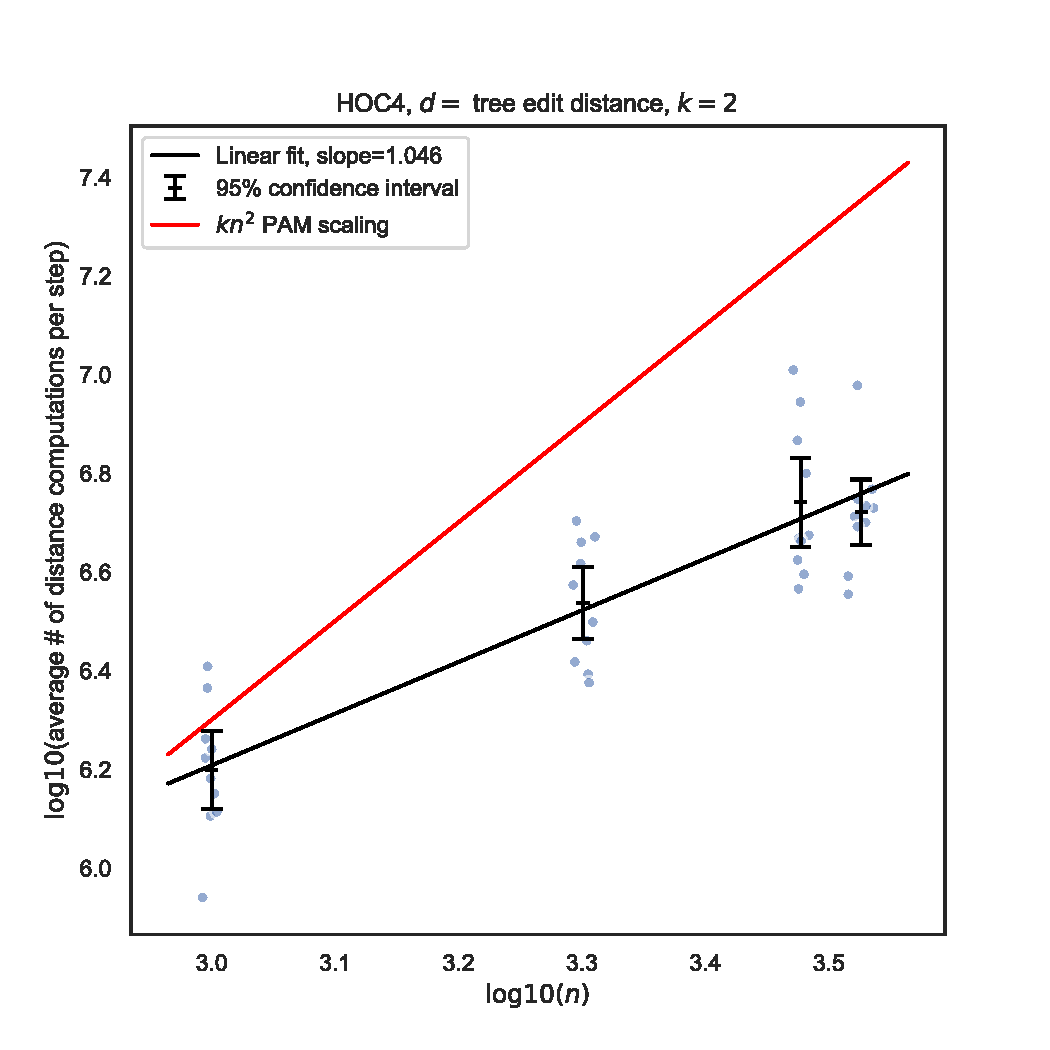
\includegraphics[width=\linewidth]{figures/HOC4-tree-k2.pdf}   
  \caption{}
  \label{fig:scaling3}
\end{subfigure}
\caption{Average number of distance calls per iteration vs sample size $n$, for (a) MNIST and cosine distance, (b) scRNA-seq and $l_1$ distance, and (c) HOC4 and tree edit distance. The plot is shown on a log-log scale. Lines of best fit (black) are plotted, as are reference lines demonstrating the expected scaling of PAM (red).}
\label{fig:scaling}
\end{figure}

%When assessing the scaling of \algnamenospace, we treat the entire BUILD step as a single SWAP iteration. Indeed, the entire BUILD procedure for the $k$-medoids problem on dataset $\mathcal{X}$ can be reduced to a single SWAP iteration for the $k+1$-medoids problem on the dataset $\mathcal{X}$ augmented with $k+1$ equal points infinitely far away from $\mathcal{X}$.

We next consider the number of distance calls per iteration as the sample size increases. 
The number of distance calls per iteration is defined as the total distance calls divided by the number of SWAP steps plus 1, where the plus 1 corresponds to the BUILD step. We choose to look at this quantity to account for different number of SWAPs for different runs, in order to provide a fair comparison. 

If the complexity is linear, then the slope would be $1$ in the log-log plot. 
Indeed, as shown in Figure \ref{fig:mods} (b-c), the slope for $k=5$ and $k=10$ are 0.979 and 0.930, respectively, indicating the scaling is linear in $n$ for different values of $k$. 

In addition, as shown in Figure \ref{fig:scaling}, the slopes of the log-log plot are 1.018, 0.899 and 1.046 for MNIST with cosine distance, scRNA-seq with $l_1$ distance, and HOC4 with tree edit distance, respectively, validating our theory that \algname takes almost linear number of distance evaluations per iteration for different datasets and different distance metrics.

% \subsection{Different distance metrics and increasing $k$ \label{subsec:mods}}

% Naturally, one might ask if \algname only demonstrates the expected speedup for a particular choice of metric for a given dataset. Figure \ref{fig:fig1} shows the scaling of the average number of distance calls in the BUILD step (Algorithm 1) and SWAP step (Algorithm 2) of \algname with $n$ for the MNIST dataset, but using cosine distance instead of $l_2$. \algname still runs in near-linear time; the slopes of the lines of best fit is 1.2 in BUILD and 1.1 in SWAP. These results suggest the algorithmic speedup of \algname is not dependence on the choice of distance metric used for a given dataset.

% Empirically, we observe that \algname exhibits almost-linear scaling for various choices of distance metric, even for the same dataset. Whereas Figure \ref{fig:scaling} (left) suggested that \algname scales linearly on MNIST when using cosine distance, Figure \ref{fig:mods} (left) suggests that \algname also scales linearly when considering $l_2$ distance on MNIST; the slope of the line of best fit is 0.979. 


% Additionally, we find that the scaling of \algname is not too sensitive to $k$, as long as $k \ll n$. Figure \ref{fig:mods} (right) demonstrates the scaling of \algname when $k$ is increased to 10; the slope of the line of best fit (0.930) still suggests roughly linear scaling in $n$.

%\mo{Mo: Add plots for MNIST,L2 k = 10 too}

